\chapter{Finite State-Machines}
\label{cha:logic}
    \tikzstyle{state} = [rectangle, draw=none, rounded corners=1mm, fill=YellowGreen,
                    text centered, anchor=north, text=white, minimum width=2.5cm, minimum height=1cm, node distance=3cm, align=center]
    \tikzstyle{condition} = [diamond, draw=none, fill=red!80,
                    text centered, anchor=north, text=white, minimum height=1cm, node distance=3cm, align=center]
    \tikzstyle{choice}=[font=\scriptsize]

    State-machines are a modeling tool to describe the behavior of a system
    in terms of \textit{states} and the transitions between them.
    Several paradigms of state-machines exist - Mealy and Moore being the notable forefathers in the field.

    In projects related to the LinkQuad quadrotor, generic state-machine
    frameworks have been developed and researched in previous projects \citep{Merz06,Wzorek11}.
    On the LinkQuad, for the purpose of this thesis, a simple state-machine engine
    was implemented.% in the \textit{CRAP} framework presented in Appendix~\ref{app:crap}.

    This state-machine is responsible for transitioning between the
    states predefined in an action sequence (a \textit{mode}), ultimately
    providing reference signals for the controller.
    Each state represents an action, which is performed repeatedly until
    a transition condition is met.
    Figure~\ref{fig:logic:statemachine} exemplifies the notation used in this chapter.

    \begin{figure}[H]
        \noindent\makebox[\textwidth]{%
            \begin{tikzpicture}[auto]
                \node (entry) {Entry};
                \node [state, right of=entry] (state1) {State 1 \\ \footnotesize{Do something}};
                \node [condition,right of=state1] (cond) {Condition};
                \node [state, right of=cond] (state2) {State 2 \\ \footnotesize{Do something else}};
                \node [right of=state2, node distance=2.5cm] (cont) {$\cdots$};
                \path[->]
                    (entry) edge (state1)
                    (state1) edge (cond)
                    (cond) edge (state2)
                    (state2) edge (cont)
                ;
            \end{tikzpicture}
        }
        \caption{State-machine example mode. An active state is repeatedly invoked until a transition condition is met. The next state is then activated.}
        \label{fig:logic:statemachine}
    \end{figure}

    In this chapter, four basic modes are presented which were implemented
    in the time-frame of this thesis.

\pagebreak
    \section{Hovering Mode}
        In the hover mode, the position of the quadrotor is recorded at
        the time of the activation, and three independent PID-controllers
        are initialized to generate reference velocities to the main controller,
        to keep the quadrotor at the place where the mode was first initialized.
        \begin{figure}[H]
            \noindent\makebox[\textwidth]{%
                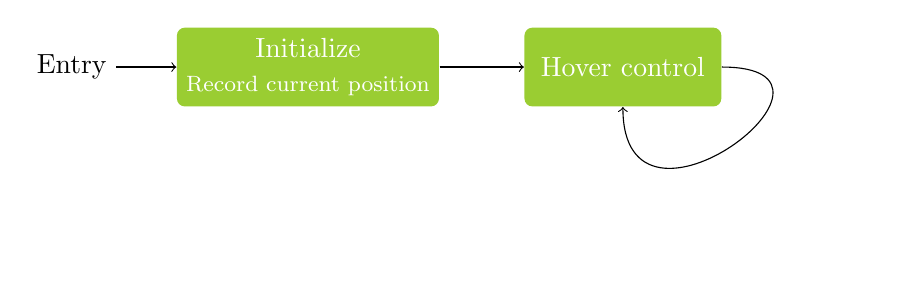
\begin{tikzpicture}[auto]
                    \node (entry) {Entry};
                    \node [state, right of=entry,text centered, align=center, node distance=3cm] (init) {Initialize \\ \footnotesize{Record current position}};
                    \node [state, right of=init, node distance=4cm] (hover) {Hover control};
                    \path[->]
                        (entry.east) edge (init.west)
                        (init.east) edge (hover.west)
                        (hover.east) edge [loop below, out=0, in=-90, distance=2cm] (hover.south);
                \end{tikzpicture}
            }
            \caption{Hovering scheme. The position of the quadrotor is recorded when the mode is activated. The hover control state is then immediately activated to keep the quadrotor in this position.}
            \label{fig:logic:hoverscheme}
        \end{figure}
        
    \section{PTAM Initialization Mode}
        By entering this mode, an automated initialization process is started to
        initialize the PTAM library and set up the transformation discussed in Chapter~\ref{cha:observer}.
        Commands are sent to the PTAM module to initialize tracking, after which
        the quadrotor should be moved sideways for the stereo
        initialization to be performed by the PTAM library.

        As part of the proposed modifications to the PTAM library, the
        initialization process is started remotely on command,
        and the video-captured motion is then monitored to determine either
        when the initialization has failed - in which case it is simply restarted -
        or when the camera has moved enough for a stable stereo initialization to be performed.

        \begin{figure}[H]
            \noindent\makebox[\textwidth]{%
            \begin{tikzpicture}[auto]
                \node [state] (notstarted) {Tracking not started};
                \node [condition, below of=notstarted] (start) {Start tracking};
                \node [state, below of=start] (dostart) {Start initial tracking};
                \node [state, below of=dostart] (started) {Initial tracking started};
                \node [condition, below of=started] (enough) {Moved enough};
                \node [condition, right of=started] (lost) {Lost};
                \node [state, below of=enough] (init) {Initialize map};
                \node [state, below of=init] (tracking) {Tracking};
                \node [condition, left of=started] (reset1) {Reset};
                \node [condition, left of=tracking] (reset2) {Reset};

                \path[->]
                    (notstarted) edge (start)
                    (start) edge (dostart)
                    (dostart) edge (started)
                    (started) edge (enough)
                    (started) edge (lost)
                    (lost.north) edge[bend right] (notstarted.east)
                    (enough) edge (init)
                    (init) edge (tracking)
                    (started) edge (reset1)
                    (tracking) edge (reset2)
                    (reset1.north) edge[bend left] (notstarted.west)
                    (reset2.north) edge[bend left] (notstarted.west)
                ;
            \end{tikzpicture}
            }
            \caption{After the commands have been sent to start the PTAM initialization routine, the quality of the tracking is monitored until a stable map initialization is deemed to be possible.}
            \label{fig:logic:ptamscheme}
        \end{figure}

    \section{Free Flight Mode}
        In the free flight mode, control reference signals for velocties
        and yaw rate are forwarded from the joystick reference provided
        over the serial interface from the user interface.

        \begin{figure}[H]
            \noindent\makebox[\textwidth]{%
                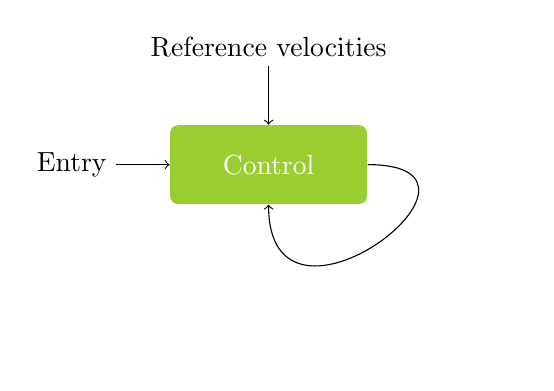
\begin{tikzpicture}[auto]
                    \node (entry) {Entry};
                    \node [state, right of=entry, node distance=2.5cm] (control) {Control};
                    \node [above of=control, node distance=1.5cm] (reference) {Reference velocities};
                    \path[->]
                        (entry.east) edge (control.west)
                        (reference.south) edge (control.north)
                        (control.east) edge [loop below, out=0, in=-90, distance=2cm] (control.south);
                \end{tikzpicture}
            }
            \caption{Free flight scheme. The free flight mode merely forwards controller reference signals received from the user interface.}
            \label{fig:logic:freeflightscheme}
        \end{figure}

    \section{Landing Mode}
        \label{ssec:logic:landing}
        There have been several studies of autonomous quadrotor landing,
        e.g. \citep{mellinger10perching,brockers:803111}.
        In \citep{brockers:803111} a landing scheme is proposed which is
        closely related to that which is proposed in this thesis.
        The algorithm used can be summarized in the following steps:
        \begin{itemize}
            \item Detection of landing site,
            \item Refinement of landing site position estimate,
            \item Descent on landing site,
            \item Landing detection.
        \end{itemize}

        In the landing site detection phase, the environment is searched for a suitable
        landing place. In \citep{brockers:803111}, landing is then performed
        on an elevated surface which is detected using video processing.
        After the landing area has been located, the position of the
        landing site - relative to the quadrotor - is filtered to increase the
        confidence of the position estimate.

        \begin{figure}[H]
            \noindent\makebox[\textwidth]{%
                \begin{tikzpicture}[auto]
                    \node (entry) {Entry};
                    \node [state, right of=entry] (halt) {Halt to hover\\ \footnotesize{Set $V_{ref}=0$}};
                    \node [condition,right of=halt] (halted) {$|V| < \epsilon$};
                    \node [state, below of=halt, node distance=2cm] (descend) {Descend \\ \footnotesize{Set $V_{ref,z} > 0$}};
                    \node [condition,right of=descend] (landed) {Landed};
                    \node [state, below of=descend, node distance=2cm] (spindown) {Spin down};
                    \path[->]
                        (entry.east) edge (halt.west)
                        (halt.east) edge (halted.west)
                        (halted) edge[loop right,in=90,out=-135] (descend.north)
                        %~ (halted.east) edge [loop right,distance=2cm, in=45,out=-45] node [choice] {No} (halted.east)
                        %~ (halted) edge [loop right,in=90,out=-135] node [choice,yshift=0.2cm] {Yes} (descend.north)
                        (descend.east) edge (landed.west)
                        (landed) edge[loop right,in=90,out=-135] (spindown.north)
                        %~ (landed.east) edge [loop right,distance=2cm, in=45,out=-45] node [choice] {No} (landed.east)
                        %~ (landed) edge [loop right,in=90,out=-135] node [choice,yshift=0.2cm] {Yes} (spindown.north)
                %       (control.east) edge [loop below, out=0, in=-90, distance=2cm] (control.south)
                    ;
                \end{tikzpicture}
            }
            \caption{Landing scheme. The landing mode consists of three stages to perform and detect landing.}
            \label{fig:logic:landingscheme}
        \end{figure}

        While the landing site position estimate converges, the quadrotor is moved to
        a position above the landing site as preparation for the Descend phase,
        where the quadrotor lowers until landing has been detected,
        using the camera feedback and other sensors to stabilize the descent.

        The landing site detection of the algorithm is not covered by
        this thesis, but the other steps of the described landing scheme
        is implemented as described by Figure~\ref{fig:logic:landingscheme}.

        \subsection{Landing Detection}
        \label{ssec:logic:landing:detection}
            In the landing detection, it must be recognized that the
            estimated position - initialized at the starting point -
            is not necessarily consistent with the true Height Over Ground (HOG)
            at the landing site. It is thus necessary to implement a more robust
            method to detect the completion of the landing procedure than simply halting at zero height.
            The proposed approach is to use the observer's estimate to determine when the movement
            has stopped; that is, when the quadrotor has reached ground.
            Detection theory, as discussed in e.g. \citep{Tornqvist08,nyberg11diagnosis},
            provides several tools for detecting the nonlinear event that
            the quadrotor can descend no further.

            In the physical model presented in Chapter~\ref{cha:observer},
            two terms is of specific interest for the detection.
            The first - and the obvious - is the altitudinal velocity.
            When sensor measurements pull this term towards zero,
            this is a first indication that the quadrotor has stopped.
            When the sensor measurements indicate a halt, the
            observer - whose motion model is oblivious to the forces imposed by the
            ground contact - will explain the lack of movement by a drastic increase in
            the estimated vertical wind velocity.
            This estimated state - the second of interest - is easily monitored
            and could be further filtered to increase detection confidence,
            or simply thresholded to detect landing.
